\documentclass{article}
\usepackage[utf8]{inputenc}
\usepackage{amsfonts}
\usepackage{amssymb}
\usepackage{graphicx}
\usepackage{hyperref}
\usepackage{amsmath}
\usepackage{pgfplots}
\pgfplotsset{compat=1.18}
\usepackage[backend=biber, style=numeric]{biblatex}
\addbibresource{references.bib}
\usepackage{titlesec}
\titleformat{\subsection}[hang]{\normalfont\bfseries}{\thesubsection}{1em}{}
\usepackage{abstract}
\usepackage[labelformat=empty]{caption}

\begin{document}
\pagenumbering{gobble}
\begin{figure}
  \centering
  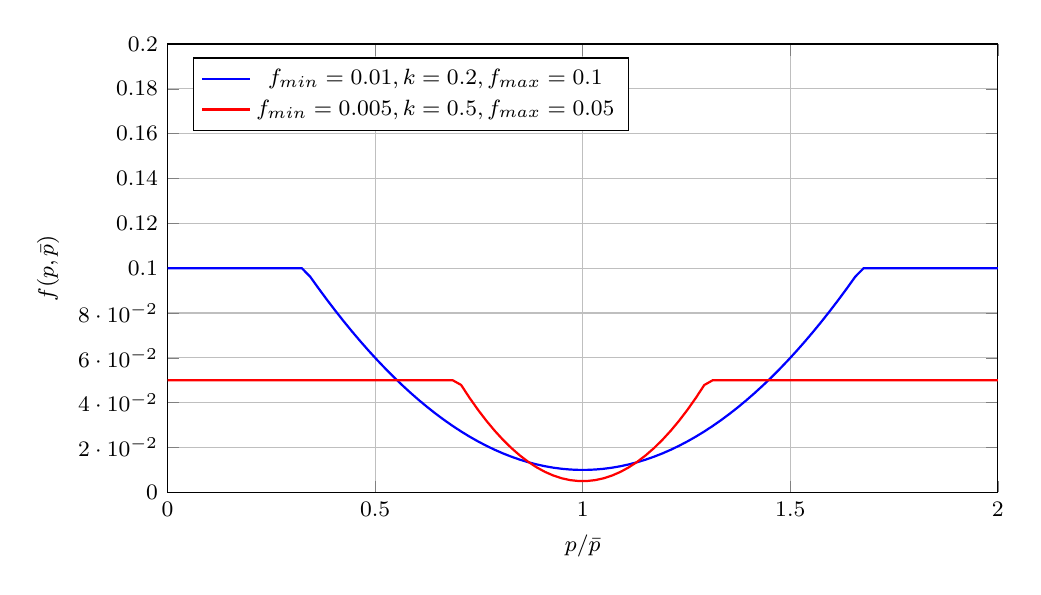
\begin{tikzpicture}
    \begin{axis}[
      xlabel={$p / \bar{p}$},
      ylabel={$f(p, \bar{p})$},
      xmin=0, xmax=2,
      ymin=0, ymax=0.2,
      xtick={0,0.5,1,1.5,2},
      ytick={0,0.02,0.04,0.06,0.08,0.1,0.12,0.14,0.16,0.18,0.2},
      legend pos=north west,
      grid=major,
      width=\columnwidth,
      height=0.6\columnwidth,
      tick label style={font=\footnotesize},
      label style={font=\footnotesize},
      legend style={font=\footnotesize},
      domain=0:2,
      samples=100,
    ]
    
    \addplot[color=blue, thick] {min(0.01 + 0.2 * (x - 1)^2, 0.1)};
    \addlegendentry{$f_{min} = 0.01, k = 0.2, f_{max} = 0.1$}
    
    \addplot[color=red, thick] {min(0.005 + 0.5 * (x - 1)^2, 0.05)};
    \addlegendentry{$f_{min} = 0.005, k = 0.5, f_{max} = 0.05$}
    
    \end{axis}
  \end{tikzpicture}
  \caption{Volatility-based swap fee with various parameter shoices}
  \label{fig:dynamic_fee_model}
\end{figure}

\end{document}